% interactapasample.tex
% v1.05 - August 2017

\documentclass[]{interact}

\usepackage{t1enc}
\usepackage[utf8]{inputenc}
\usepackage{epstopdf}% To incorporate .eps illustrations using PDFLaTeX, etc.
\usepackage[caption=false]{subfig}% Support for small, `sub' figures and tables
%\usepackage[nolists,tablesfirst]{endfloat}% To `separate' figures and tables from text if required
%\usepackage[doublespacing]{setspace}% To produce a `double spaced' document if required
%\setlength\parindent{24pt}% To increase paragraph indentation when line spacing is doubled

%\usepackage[longnamesfirst,sort]{natbib}% Citation support using natbib.sty
%\bibpunct[, ]{(}{)}{;}{a}{,}{,}% Citation support using natbib.sty
%\renewcommand\bibfont{\fontsize{10}{12}\selectfont}% To set the list of references in 10 point font using natbib.sty

\usepackage{subfiles}
\usepackage{standalone}
\usepackage{url}

\usepackage[natbibapa,nodoi]{apacite}% Citation support using apacite.sty. Commands using natbib.sty MUST be deactivated first!
%\setlength\bibhang{12pt}% To set the indentation in the list of references using apacite.sty. Commands using natbib.sty MUST be deactivated first!
%\renewcommand\bibliographytypesize{\fontsize{10}{12}\selectfont}% To set the list of references in 10 point font using apacite.sty. Commands using natbib.sty MUST be deactivated first!

\usepackage{wasysym} % male and female symbols
\usepackage{floatpag}
\usepackage{float}
\usepackage{changepage}
\usepackage{threeparttable}
\usepackage{tcolorbox}
\usepackage{graphicx,import} %for pdf_tex image

\usepackage[section]{placeins} % floating barrier

\newcommand{\dq}{"}

% ##################
% Tikz 

\usepackage{tikz}
\usepackage{tikz-3dplot}
\usetikzlibrary{decorations.pathmorphing,patterns,positioning,calc,intersections,through,backgrounds,arrows,automata,shadings,decorations.pathreplacing}


\tikzset{
    state/.style={
           rectangle,
           rounded corners,
           draw=black, very thick,
           minimum height=2em,
           inner sep=6pt,
           text centered,
           }, >=stealth',
}

% ####################



\begin{document}

%\articletype{ARTICLE TEMPLATE}% Specify the article type or omit as appropriate

\title{Chracterizing successful participants in ScienceOlympiads -- Evidence from the PhysicsOlympiad}

\author{
\name{Peter Wulff\textsuperscript{a}\thanks{CONTACT Peter Wulff. Email: peter.wulff@uni-potsdam.de}, Stefan Petersen\textsuperscript{b}, Melanie Keller\textsuperscript{b}, Tim H\"o{}ffler\textsuperscript{b}, and Knut Neumann\textsuperscript{b}}
\affil{\textsuperscript{a}Physics Educational Research Group, University of Potsdam, Karl-Liebknecht-Stra\ss e 24/25, 14476 Potsdam-Golm \\ \textsuperscript{b}Leibniz Institute for Science and Mathematics Education, Olshausenstrasse 62, 24118 Kiel, Germany}
}

\maketitle

\begin{abstract}
Given the need for high-achieving students to engage in science, technology, engineering, and math (STEM), this study seeks to characterize successful students in the Physics Olympiad as a means to enable future educational efforts to be more in congruence with the characteristics of the students. On the basis of the expectancy-value model of achievement motivation and research in expertise, $N=141$ students were tracked in their engagement with the Physics Olympiad and administered appropriate motivational and cognitive constructs. The dependent outcome variable was the success the students had in their participation in the Physics Olympiad. Results indicate that successful students can be characterized through high skills in physics problem solving and positive motivational attributes, namely a high expectation to be successful in the Physics Olympiad. These results pave the path to more transparency for what comprises expertise in domains like physics such that designated educational efforts can motivate and foster more students.
\end{abstract}

\begin{keywords}
Problem solving, Physics competitions
\end{keywords}

\maketitle

\section{Introduction}

Enrichment programs such as the ScienceOlympiads are means to identify and promote talented students in science, technology, engineering, and math (STEM). These programs proceed in subsequential stages where students solve increasingly complex domain-specific problem and eventually meet and compete with one each other \citep{Petersen.2017}. Amongst the most successful students, a national team is chosen, comprising about five students, who compete on an international level against students from more than 80 countries in the Physics Olympiad. Federal government and the STEM community endorse these means as viable instruments to foster talented students \citep{KMK.2009,Petersen.2017}--and educational researchers in gifted programs motivated the necessity of ScienceOlympiads (and programs alike) as a viable complementary to regular schools that have limited capacities to provide resources for talented students \citep{Reis.2010}. Besides these goals, research is scare on these programs \citep{Ziegler.2004}.

The available studies document that successful candidates report a positive impact on their future job aspirations in STEM through programs such as the ScienceOlympiads \citep{Feng.2001,Oswald.2004,Subotnik.1993}. Further research suggests that these programs can have effects for training skills related to cognitive abilities and related to beliefs such as developing interest and motivation of students towards STEM \citep{Oswald.2004,Aljughaiman.2012,Wai.2010,Marsh.1995}. Due to the broad motivation of enrichment programs (foster gifted students) and the self-selective mechanisms for participation, other studies sought to characterize participants in these programs in order to advance an understanding for characteristics of successful participants. \cite{Urhahne.2012} found for the ChemistryOlympiad that previous participation was the best predictor for success in this competition and also expectancy of success distinguished successful participants from less successful participants \citep[similar findings in:][]{Stang.2014}. Taken together, the above studies suggest that successful students in programs such as the ScienceOlympiads show advantageous dispositions in cognitive variables such as general cognitive abilities, and that more successful students display advantageous beliefs such as a high expectancy of success towards the competition.

However, two problems arise in the context of the above studies. First, even though cognitive abilities appear to be particularly predictive for success in these programs, operationalization of domain specific abilities is insufficient so that it remains unclear to what extent domain-specific cognitive abilities are characteristic of successful participants in these programs. Second, no such analyses have been done for the Physics Olympiad. Physics is often suggested to be particularly heavy in content dependency such that characterizing successful participants in the Physics Olympiad might hinge on an integrative assessment of both cognitive variables and beliefs.


\section{Modelling success in ScienceOlympiads}

Applied to the context of the Science Olympiads, \cite{Urhahne.2012} applied the expectancy-value model of achievement motivation in order to explain variance in success for the participants. The expetcancy-value model outlines two proximal causes for achievement related choices and performance in a situation: expectancy to be successful in a task (''Can I do this?'') and the values brought towards performing the relevant tasks (''Do I want to do this?'') \citep{Eccles.1983}. The model has been empirically validated in multiple contexts such as occupational choices REF, academic choices in school \citep{Koller.2000} and ScienceOlympiads \citep{Urhahne.2012}. 

Expectancy of success and values towards the context (e.g., ScienceOlympiad) are also influenced by other multiple variables that commonly in talent research relate to cognitive dispositions (stable and vairable), affective/motivational variables, and external motivational moderators \citep[e.g.,][]{Ziegler.2009,Heller.2002}. Regarding cognitive dispositions, it has been implicated from the inception of talent studies that general cognitive abilities successful from less successful students--talent was even defined through scores in general cognitive abilities \citep{Rost.2010}. Later on, incited by studies in domains such as chess and physics, researchers acknowledged that domain-specific skills such as problem solving are the characteristic features that distinguish successful from less successful students in a domain \citep{Chi.1981}. Today, it is clear that successful students in a domain invest enormous amounts of deliberate practice to master a domain \citep{Simon.1983}. Consequently, domain-specific abilities are essential for characterizing successful students in programs such as the ScienceOlympiads. 

Affective and motivational variables can be characterized to be beliefs about oneself that potentially impact goal-directed behavior in that domain \citep{Rheinberg.2012}. There is contentious debate, what essential affective and motivational aspects direct human behavior, but competence, belongingness, and interest are conceptualized in most models \citep{Deci.2000,Hazari.2010}. \cite{Bandura.1997} presented a broad program outlining the importance of self-efficacy beliefs (closely linked to competence) and educational outcomes such as positive attitudes towards performance. Regarding belongingness, \cite{Baumeister.1995} muster evidence that humans perform better when they feel accepted and related to people in the respective community. \cite{Good.2012} link the sense of belonging for students to academic choices in mathematics. Finally, domain interest is linked to positive learning outcomes and academic choices in the domain \citep{Krapp.2002,Hazari.2010}. External motivational moderators can be conceived of as social support by meaningful others. For example, the attitudes of peers, teachers, and parents are an important facilitator for achievement in an academic competition \cite[e.g.,][]{Urhahne.2012}.

While for the ChemistryOlympiad and the BiologyOlympiad first results with regards to characterization of successful participants are available \citep{Urhahne.2012,Stang.2014}, such results are missing for the PhysicsOlympiad. Furthermore, instruments for measuring domain-specific abilities are missing such that the characterization of successful participants to date remains incomplete. Consequently, two research questions are addressed in this study:
\begin{enumerate}
\item To what extent can cognitive variables (general cognitive abilities and domain-specific abilities) characterize successful students in the PhysicsOlympiad?
\item To what extent do affective/motivational variables additionally explain success in the PhysicsOlympiad?
\end{enumerate}

\section{Design}

Characterizing successful students in the PhysicsOlympiad suggests a design where students' performance in the competition is registered and where (in the optimal case all) participating students respond to the above outlined constructs. This is facilitated through two measurement times where students respond to items on an online platform. As soon as participants registered in the PhysicsOlympiad registration platform (each year approx. 1000 students do so \citep{Petersen.2017}), these students received an invitation to participate in an online survey that accompanies them throughout their participation in the competition and where the students could win prices through participation. Participation was entirely voluntary, anonymous, and independent from the competition participation. This information was given to the students prior to their participation. Throughout the students' participation advancing rounds of the online questionnaire were unlocked and open for participation. 

At some point during their participation in stage 1 of the PhysicsOlympiad (where students do homework problems and hand them in to their physics teacher) the participants received an email that the first online questionnaire was open for participation. Students who did not participate received reminder emails until at some point the first questionnaire was closed. In the parallel competition the students received a notification whether they advanced through stage 2 in the competition. After this notification the second online questionnaire was unlocked for participation. This procedure repeated until after stage 4. The relevant design for the current study is displayed in Figure \ref{Design}.

\begin{figure}
\centering
\import{../../img/}{design.pdf_tex}
\caption{Design for measurements of different variables throughout the PhysicsOlympiad.}
\label{Design}
\end{figure}


\section{Instruments}

Instruments are employed with regards to cognitive, affective/motivational, and external motivational variables. 

\subsection{Cognitive variables}

Cognitive variables that potentially predict success in programs such as the ScienceOlympiads are general cognitive abilities. A simplified version of Carroll's hierarchical theory of cognitive abilities is the radex model where quantitative/numerical, spatial/pictorial, and verbal/linguistic abilities are differentiated \citep{Snow.1997}. Students that excel in STEM show generally high cognitive abilities. For example, \cite{Wai.2009} find that less than $10$ percent of those holding a STEM-PhD were below the top quartile in cognitive ability (comprising spatial visualization in 2D and 3D, mechanical reasoning, and abstract reasoning) during adolescence, and their data supports the conclusion that the importance of spatial ability for STEM increases with more advanced degrees (bachelor, master, PhD). Graduates in physical sciences such as engineering range among the top performers in cognitive abilities \citep[see also:][]{Shea.2001}. ''STEM disciplines place a premium on nonverbal ideation indicative of quantitative and spatial reasoning'' \citep{Lubinski.2010}. Consequently, this study focuses on quantitative and numerical abilities, because of its central importance for STEM \citep{Wai.2009}. A sample item from the test for general cognitive abilities in numerical scale asks: ''What quantity is bigger: $\sqrt{100}$ or $50$?'' 34 items were used from the quantitative and numerical scales from the test for general cognitive abilities \citep{Heller.2007}. Only items that were applicable for grades 9 to 12 were retrieved to build a sum score for each participant. This gives an approximation of general cognitive abilities with regards to a norm, rather than an age adaptive measure as is usually done in intelligence testing.


Besides general cognitive abilities, indicative of success in the PhysicsOlympiad is likely to be physics problem solving abilities \citep{Maloney.2011}. Physics problem solving is laregly based on prior knowledge \citep{Bhaskar.1977}, where commonly factual knowledge (declarative), strategic (procedural) knowledge, and conditional knowledge are necessary \citep{Anderson.1996}, which are chunked in problem schemata \citep{Reinhold.1999}. Knowledge  and problem schemata are applied in different phases of problem representation, strategy selecton, solution, and verification of solution \citep{Polya.1945,Mayer.2013}. Experts carefully conduct a qualitative problem analysis prior to solving a problem based on the fundamental principles involved \citep{Larkin.1980,Chi.1981}. Expert knowledge is furthermore applicable in new situations (conditionalized) \citep{Simon.1980,Glaser.1992}, because experts categorize problems by basic concepts (deep structure), whereas novices categorize problems by surface features such as ''is a pulley involved?'' \citep{Chi.1981,Schwartz.2015}. Novices have problems to recognize and reflect upon the assumptions that predicate the solution to a problem. \cite{Reif.1992} report that novice students showed deficient applicability conditions for concepts and thus the use of the concepts was flawed.

Physics problem solving ability, here, entails the ability to apply explicit, structured knowledge in various problem situations to achieve a desired goal state. \cite{Leonard.1996} propose a measure for physics problem solving ability that assesses the strategies that students use to solve problems. Strategies, as the authors use the term, entail the concept to solve the problem, a justification for why the concepts can be applied (i.e., conditional knowledge), and a procedure by which the concept is applied. The authors emphasize the role of conceptual knowledge that is important for physics problem solving and the idea that problem solving strategies shall be established before applying mathematics. On the basis of the aforementioned definition of physics problem solving ability, a similar rationale as in cite{Leonard.1996} was adopted in this study in order to measure physics problem solving ability. Students were asked to write down the physics ideas that they would use to solve the well-defined physics problem without going through the whole problem solution process (i.e., leaving out problem representation and mathematical routines). Consequently, the items provided the students space to construct their understanding and give context to their thoughts \citep{Hammann.2014}. In order to make clear to students what was meant with the prompt, an example was provided to all students that they read through. Afterwards, four physics problems (two mechanics, two electro-magnetism) followed that each had a certain context and well-defined solution plans.

A theory-based coding rubric was utilized for scoring the responses. \cite{Docktor.2016} developed a similar coding rubric for students' written solutions for physics problems. Not all of the five categories were adopted for the measure in this study, so that the coding rubric comprised the categories concept, execution, context, and detail. Concept entails information if students provide all relevant concepts that are necessary for solving the problem (physics approach in \cite{Docktor.2016}). Execution entails information about the comprehensiveness of the response (logical progression). Context reflects the assumptions and conditions for applying the concepts (specific application of physics) \citep{Fortus.2009}, and, finally, detail detected when students' interspersed their response with an elaboration of the concepts such as through mathematical formulas where the relevant variables became clear. Furthermore, these aspects also relate to the strategy definiton in \cite{Leonard.1996}. Similar to the rubric by \cite{Docktor.2016}, all categories were graded with $0$ to $2$ points. Moreover, concept and context could be graded negative ($-1$) when a concept was wrong (e.g., when students used magnetic force instead of electric force in a problem). For concept the full score was given when the student response included all concepts that were central to the respective problems. Execution pertained the presentation of the physical ideas. If the sentences were understandable (not only two-word phrases) and logically connected, full credit was given. Full credit for detail was awarded when all relevant variables in the concepts were identified. Full credit for context was given when important assumptions and boundary conditions were identified (e.g., frictionless slide). Note that the categories are not idependent of each other. As a consequence, we aggregated the score for each student to an overall measure which is henceforth called ability of problem conceptualization, because a full credit (i.e., $8$ points for each problem) would indicate that the student has all the relevant analyses correct that would count for successful physics problem solving.

Four physics problems were presented to the students that are related to two fundamental physics topics that are encountered throughout physics: mechanics and electro-magnetism. Knowledge for gravitational and electro-magnetic force, momentum, and energy conservation were necessary to solve all problems. A sample problem from mechanics reads:

\begin{tcolorbox}
A mass runs through a looping (see picture below). The mass starts from a heights above the highest point of the looping. The movement is frictionless.

Determine the minimal necessary heights for the mass, so that the mass can run through the looping without falling down. Assume that the mass does not slip and that it is a point mass.

\textit{Describe how you would solve this problem and what physics ideas you would use to solve it. Try to write full sentences.}

\begin{center}
\subfile{../../img/sample_problem}
\end{center}
\end{tcolorbox}

An expert answer for this open-ended problem looked as follows: 
\begin{quote}
The centrifugal force at the highest point of the looping needs to be equal with the weight: $(m*v^2)/r=m*g$. In order to figure out how high the starting point needs to be, we calculate the initial speed that he needs in order to pass the looping and with the energy conservation law we determine the height: $v=\text{sqrt}(g*r), \; mgh=m/2*v^2 h=0.5r+2r$ (height of the looping) $h=5/2R$.

% Die Fliehkraft muss am h\"o{}chsten Punkt des Looping, genau so gross [sic!] sein wie die Gewichtskraft: $(m*v^2)/r=m*g$. Um herauszufinden wie hoch der Startpunkt sein muss, berechnen wir zun\"a{}chst die Anfangsgeschwindigkeit die er braucht um das Looping zu schaffen und \"u{}ber den Energieerhaltungssatz daraus die H\"o{}he $h$: $v=\text{sqrt}(g*r), \; mgh=m/2*v^2 h=0.5r+2r$ (H\"o{}he Looping) $h=5/2R$.
\end{quote}

In this answer, $2$ points were given for the concepts (equilibrium of forces and energy conservation). Furthermore the student's answer is coherent and it is easy for the reader to follow ($2$ points for execution). Details are given through the correct formulas. Missing points appear for the context, because the student does not include a reflection of boundary conditions in the response. A novice response, were no credit is awarded, looked like this:
\begin{quote}
I would recognize the ascent of the trajectory and the height of the looping. Besides, I think the mass of the object is crucial. At first I would calculate the velocity or acceleration on the initial path and the velocity with which the object enters the looping. With the gravitational acceleration and the initial acceleration you could calculate which acceleration and initial height is necessary that the object does not fall out the looping.

%Ich würde die Steigung der Bahn und die Höhe des Loopings beachten. Außerdem ist meiner Meinung nach die Masse des Körpers entscheidend. Als erstes würde ich die Geschwindigkeit bzw. Beschleunigung auf der Startstrecke berechnen und die Geschwin\-digkeit, mit der der Körper in den Looping eintrifft. Aus der Gravitationsbeschleunigung und der Anfangsbeschleunigung könnte man ausrechnen, welche Beschleunigung und somit Anfangshöhe erforderlich ist, damit der Körper nicht aus dem Looping fällt.
\end{quote}

In order to validate the ratings, two raters (first author and physics undergraduate student with extensive experience in math and physics) that were familiarized with the problems coded the student responses. Both raters were trained to score the responses with regards to the rubric. All student responses were scored. When both raters disagreed, the disagreements were discussed and eventually a consensus was reached with regards to the final scoring.

\subfile{../../interrater/interrater}

Finally, a measure for more general physics problem solving abilities was employed that was utilized in other gifted research as well \cite{Heller.2007}. Keeping the same physics problem solving ability definition as above, this measure is more closely linked to an intuitive understanding of physics systems. Students were given multiple choices as response alternative and had to choose the correct answer. A sample item can be seen in Figure \ref{APT} (correct answer is C). Overall, this test comprises 15 items (each multiple choice with each 5 responses) that had to be solved in 6 minutes. Sum scores were retrieved for students.

\begin{figure}
\centering
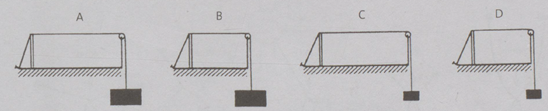
\includegraphics{../../img/APT.png}
\caption{Sample item from general physics problem solving abilities test from \cite{Heller.2007}. Choice E was the neutral choice ''Cannot be decided.''}
\label{APT}
\end{figure}

\subsection{Affective/motivational variables} 
%weiter 
Affective/motivational and external motivational variables are gleaned from the expectancy-value model and further research on motivated behavior. In particular, the expectancy of success towards enrichment programs was found to be a relevant factor for predicting success in enrichment programs \citep{Urhahne.2012}. These variables are more reactive and sensitive to individual differences in experiences and personality. 

The expectancy-value model of achievement motivation predicts also that values towards tasks in the domain are relevant for engagement. However, these effect do only show up partially (for utility value) in reality \citep{Urhahne.2012}.

A related construct to expectancy of success in the PhysicsOlympiad is the self-efficacy in physics (i.e., the perception to be able to solve physics problems). Self-efficacy is a predictor for school success \citep[e.g.,][]{Britner.2006}. 

Of yet unclear importance is the sense of belonging to the domain. It is documented that sense of belonging (the perceived belonging to a domain) is important for students to build the intention to study STEM \citep{Good.2012}, however, it is unclear if sense of belonging can explain further variance between students who engage in an Olympiad, i.e., students who already identify with the domain.


\subfile{../../analyses/instruments}


\section*{Acknowledgement(s)}


\section*{Disclosure statement}

We are not aware of potential conflicts of interest that relate to the results reported in this study.



\newpage

\bibliographystyle{apacite}
\bibliography{../../bibliography/bib}


\newpage
\section{Appendices}

\appendix



\end{document}
